\input preamble.tex
\noindent
\section*{Industrielektronikk Øving 04 - To motstandere i parallell}

I denne øvingen skal du koble to motstander i parallell.

\noindent \begin{center}
\begin{figure}[H]
\noindent \begin{centering}
%\includegraphics[angle=90,width=16cm]{\string"tegninger/Elektroteknikk - Breadboard\string".pdf}\vspace{2cm}
\par\end{centering}
\noindent \begin{centering}
%\includegraphics[width=16cm]{\string"tegninger/Elektroteknikk - koblingsbrett\string".jpg}
\par\end{centering}
$$\includegraphics[width=10cm]{./lIndustrielektronikk04.eps}$$
\end{figure}
\par\end{center}

\subsubsection*{Utstyr du trenger}
\begin{itemize}
\item Labbrettet
\item Motstand med en verdi på 2700$\Omega$ (2k7) $R_1$
\item Motstand med en verdi på 3300$\Omega$ (3k3) $R_2$
\item Multimeter
\end{itemize}

\subsubsection*{Oppgaven}
Koble de to motstandene i parallell til strømforsyningen og tegn et skjema over oppkoblingen
\begin{enumerate}
		
		\item Regn ut strømmen i hver av motstandene
		\item Mål ut strømmen i hver av motstandene
		\item Mål spenningen over hver av motstandene
		\item Koble et ampermeter i serie med LED-en og mål strømmen igjennom LED-en
\end{enumerate}

\subsubsection*{Innlevering}

Skriv en labrapport og lever på OneNote\\
\underbar{file ./lIndustrielektronikk04.tex}
\vskip 5pt 

\end{document}

